\section{问题三：由全域含水率约束确定干燥时长}
\label{sec:q3}

\begingroup
% Local spacing accommodates the added introduction without changing text size.
\setlength{\parskip}{2pt plus 1pt minus 1pt}
\setlength{\abovedisplayskip}{8pt plus 2pt minus 2pt}
\setlength{\belowdisplayskip}{8pt plus 2pt minus 2pt}
\setlength{\abovedisplayshortskip}{6pt plus 2pt minus 1pt}
\setlength{\belowdisplayshortskip}{6pt plus 2pt minus 1pt}
问题三在问题二变物性热质耦合模型的基础上，进一步确定满足含水率要求的干燥时长。
本问保持控制方程、物性关系与环境边界不变，沿用同一初态下的温湿联合轨迹。
在一维径向模型中，以全径向最大含水率严格低于$0.15\unit{kg/kg}$为终止要求，
不以表面含水率或截面平均值代替最大值。先通过下降穿越检测与括区求根定位候选等号根，
再以径向重构极值复核；结合网格加密和独立积分对照设置经验数值余量，
选取并复核严格满足阈值要求的执行点，给出所设环境条件下的模型干燥时长与径向含水率分布。
求解流程见图\ref{fig:q3-workflow}。

\begingroup
\setlength{\intextsep}{10pt}
\begin{figure}[H]
\centering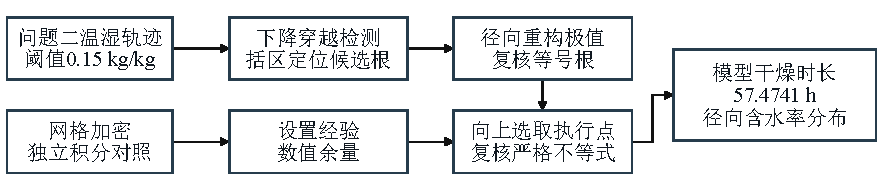
\includegraphics[width=\linewidth]{figures/q3_white/q3_workflow.pdf}
\caption{问题三的一维径向终点判定流程}
\label{fig:q3-workflow}
\end{figure}
\endgroup

\subsection{终止判据与长时计算}

问题三要求药材各处的干基含水率严格低于
$C_{\mathrm{lim}}=0.15\unit{kg/kg}$。
本文沿用问题二的附录3物性、初态和环境条件，
由同一温湿联立轨迹确定终点，而不以表面含水率或截面平均值代替最大值。
因此，本问直接沿用式\eqref{eq:q2-radial}的控制方程及
式\eqref{eq:q2-semidscrete}、\eqref{eq:q2-robin}的离散闭合，
新增的求解任务是从时间轨迹中定位满足全径向约束的执行点。
在一维径向近似中定义
\begin{equation}
 M_1(t)=\max_{0\le r\le R_0}C(r,t),\qquad
 M_1(t_{*,3})=C_{\mathrm{lim}}.
 \label{eq:q3-event}
\end{equation}
所取事件为结束附近的下降穿越。
等号根是严格达标时间集合的边界，根本身不满足题设严格不等式；
有限圆柱中“各处”的含义则由后述二维计算另行检验。

附件1仅覆盖前4\unit{h}，长时计算需延拓环境。
本文保持前述末小时61点算术均值平台，
即环境温度49.9989344262\celsius、有效边界值
$b=0.04998754098\unit{kg/kg}$。
该平台是假设的后续工况，不是4\unit{h}以后的观测记录。
温度和含水率始终按式\eqref{eq:heat}--\eqref{eq:boundary}联立推进，
不在温度接近环境后直接将温度场替换为常数。

随着含水率降低，扩散系数中的
$\exp(-0.45/C)$迅速减小，长时低含水率阶段需要保留局部非线性通量。
令
\begin{equation}
 \begin{aligned}
 a_3(T)&=2.4\times10^{-3}
 \exp\!\left[-\frac{3850}{T+273.15}\right],\\
 F_3(C)&=\int_0^C\exp(-0.45/s)\,\dd s,\qquad
 D\nabla C=a_3(T)\nabla F_3(C).
 \end{aligned}
 \label{eq:q3-primitive}
\end{equation}
采用80阶Chebyshev配点和隐式Radau方法推进，表面状态由Robin条件联立确定。
式\eqref{eq:q3-primitive}只改写通量，不改变题给扩散系数。
临界附近同时检查径向重构极值和边界值，确认最大含水率位于轴心。
空间加密与不同隐式时间方法作为交叉核验，
规定表格和完整结果均由同一未舍入轨迹生成。

\subsection{由重构空间极值到时间事件}

令$P_U(x,t)=\sum_{j=0}^N F_3(C_j(t))\ell_j(x)$为包含表面状态的
原函数插值多项式，$x=(r/R_0)^2$。在$P_U>0$的物理解支上，含水率重构为
$C_N(x,t)=F_3^{-1}[P_U(x,t)]$。由于$F_3'(C)>0$，
有$\partial_x C_N=\partial_xP_U/F_3'(C_N)$，故两者的内部驻点相同。
每一时刻的极值候选集为
\begin{equation}
 \mathcal X(t)=\{0,1\}\cup
 \{x\in(0,1):\partial_xP_U(x,t)=0\}.
 \label{eq:q3-extrema-candidates}
\end{equation}
求出式\eqref{eq:q3-extrema-candidates}中的全部实根，并比较候选点值，得到
\begin{equation}
 \widehat M_1(t)=\max_{x\in\mathcal X(t)}C_N(x,t)
 =F_3^{-1}\!\left[\max_{x\in\mathcal X(t)}P_U(x,t)\right].
 \label{eq:q3-reconstructed-max}
\end{equation}
该式确定的是重构一维场的最大值；重构误差及与连续方程的差异仍需
数值加密检验，不能把多项式极值的求全等同于连续模型严格误差为零。

实际程序先以内部节点事件$g_{\rm node}(t)=\max_{j<N}C_j(t)-C_{\rm lim}$
检测下降穿越。当相邻接受步满足
$g_{\rm node}(t_a)>0$、$g_{\rm node}(t_b)\le0$时，利用Radau的步内连续插值
对$g_{\rm node}(t)=0$作Brent括区求根，再在候选根和执行点按
式\eqref{eq:q3-reconstructed-max}复核，并用根两侧节点值检查下降穿越。
本算例确认根与执行点的重构最大值均位于轴心，节点候选根才可用于所述径向终点。
若重构出现更湿的内部点，就必须重新定位事件，不能直接接受节点根。

为解释时间裕量的尺度，在根附近作一阶展开：
\begin{equation}
 \widehat M_1(t_*+\delta t)-C_{\rm lim}
 \approx\dot{\widehat M}_1(t_*)\,\delta t,
 \qquad
 |\delta t|\approx\frac{|\delta M|}{|\dot{\widehat M}_1(t_*)|}.
 \label{eq:q3-local-event-scale}
\end{equation}
这里$\delta M$为含水率的局部数值差。已有事件记录给出末期斜率约
$-2.9128\times10^{-7}\unit{(kg/kg)/s}$；因此显示到四位小数的0.1500
不能支持亚秒级的达标判定。式\eqref{eq:q3-local-event-scale}仅作局部误差尺度
解释，正式时间预算仍取自网格与时间方法对照，不能由该线性近似给出严格界。

\subsection{结束时长与径向水分分布}

一维模型的临界根为
$t_{*,3}=206906.389932328\unit{s}$，即约57.4739972\unit{h}。
为区分数值根、执行点和四位小时显示值，
取显示时间量子$\Delta t=0.0001\unit{h}=0.36\unit{s}$，
并按空间、时间及独立方法差异设置
$\varepsilon_{t,3}=0.03\unit{s}$的经验数值余量，选择
\begin{equation}
 t_{\mathrm{exec},3}
 =\Delta t\left\lceil
 \frac{t_{*,3}+\varepsilon_{t,3}}{\Delta t}\right\rceil
 =206906.76\unit{s}
 =\boxed{57.4741\unit{h}}.
 \label{eq:q3-execution}
\end{equation}
在该实际时刻重新代入未舍入一维场，得到
\begin{equation}
 M_1(t_{\mathrm{exec},3})
 =0.149999892208\unit{kg/kg}<0.15\unit{kg/kg}.
 \label{eq:q3-end-moisture}
\end{equation}
执行点比临界根晚约0.3701\unit{s}。
这里的经验余量用于当前方程的数值选择，
不含环境、边界映射和物性假设的不确定性，也不是实验安全上界。

题设表5要求的每6\unit{h}及结束时刻的径向含水率见表\ref{tab:q3-moisture}。
18\unit{h}时，表面已降至0.0845\unit{kg/kg}，
轴心仍为0.2988\unit{kg/kg}；54\unit{h}时轴心仍为0.1539\unit{kg/kg}。
因此，表面先达到要求并不能作为全体材料的终止依据。
末期水分向低湿表面迁移，而局部扩散系数随含水率下降，
共同形成中心缓慢趋近阈值的尾段。

\begin{table}[htbp]
 \centering
 \caption{题设表5：固定半径时的径向干基含水率（\unit{kg/kg}）}
 \label{tab:q3-moisture}
 \small
 \input{tables/q3_moisture.tex}
\end{table}

完整的\texttt{result3.xlsx}以60\unit{s}为间隔、0.1\unit{cm}为径向间隔输出，
并在最后一个完整分钟206880\unit{s}之后补入执行点206906.76\unit{s}。
末行轴心显示为0.1500，是式\eqref{eq:q3-end-moisture}的四位舍入值；
达标判断使用未舍入场而不使用表格显示值。
160阶空间加密参考和另一隐式时间方法在全部72429个规定水分输出上四位一致，
\mbox{其中空间加密参考}与正式轨迹的最大未舍入差约
$9.33\times10^{-9}\unit{kg/kg}$。
该结果支持已选方程的数值稳定性，不替代物理参数验证。

\begin{figure}[htbp]
 \centering
 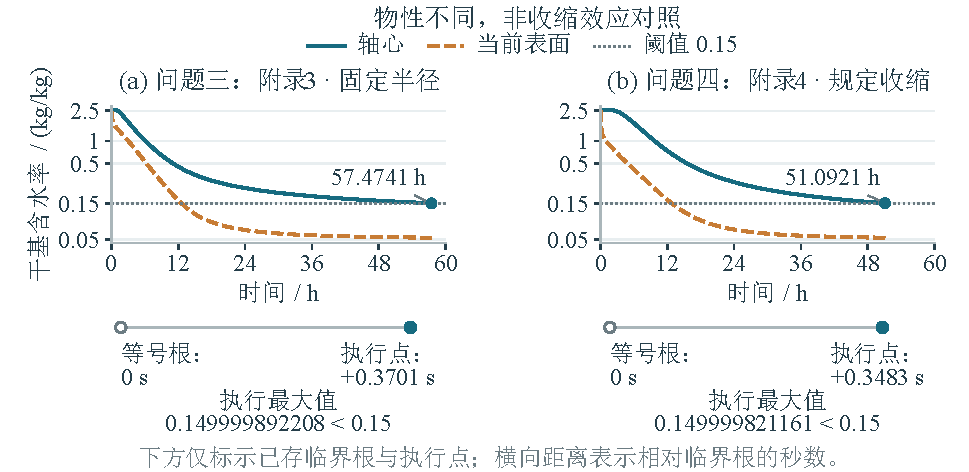
\includegraphics[width=0.93\textwidth]{figures/legibility_process/q3_q4_drying.pdf}
 \caption{问题三（左）与问题四（右）的干燥过程与事件判定。上排为一维径向有效模型的轴心、当前表面含水率演化。
 纵轴为对数刻度，水平线为0.15\unit{kg/kg}阈值，终点标记对应各自正式执行时刻。
 下排以各自临界根为时间原点，仅标示已存临界根与执行点，并列出执行最大值。
 两问采用各自附录物性，问题四另施加观测半径历程，
 因而曲线差异不能全部归因于收缩。}
\label{fig:q3-q4-drying}
\end{figure}

图\ref{fig:q3-q4-drying}上排展示表面先失水、轴心控制尾段的过程；下排将等号临界根与已选执行点分开，时间差直接取自原事件记录。

\subsection{有限圆柱检验与工况条件}

为检验“各处”的空间含义，在长度0.25\unit{m}的有限圆柱上增加轴向传递，
侧面与端面保持相同物性和交换系数。
以80个径向区间、256个轴向区间的同网格一维/二维配对计算比较事件根，
二维比配对一维提前约7.4740\unit{s}。
这一差值用于识别端部效应，不能把粗网格二维绝对根
直接替代精细一维根。

\Needspace{6\baselineskip}
再从临界附近已保存的二维场推进至式\eqref{eq:q3-execution}的执行时刻，
得到全节点最大含水率$0.149998606290\unit{kg/kg}$，
最湿点位于中截面轴心，离散场已经达标。
该节点结果与配对根差支持$57.4741\unit{h}$的工程保守方向；
局部续算仍继承前史离散误差，尚不构成连续二维域的严格数学误差界，
也不将该时长解释为精确的二维最短时间。
上述证据层级集中见第\ref{sec:limitations}节。

后段环境对终时的影响大于末位数值差。
例如，在相同4\unit{h}初始全场和其余参数下，
将之后温度平台降低1\unit{K}，事件根由约57.4740\unit{h}延至59.3413\unit{h}；
升高1\unit{K}则变为55.6884\unit{h}。
该单因素情景为人为设定而非观测误差范围（见第\ref{sec:environment-scenarios}节）。
故57.4741\unit{h}应与环境平台和有效气固边界共同报告，
不能仅凭小数位数给出真实工况下的确定性保证。

\endgroup
